\section*{Reciprocity \& Network Effects}
\label{neteffects}
In studies of social and economic behavior, direct reciprocity -- the notion that actors learn to ``respond in kind" to one another -- is argued to be an essential component of behavior.\footnote{For example, see \cite{bolton:1998, charness:2002, charness:2004, cox:2007, cox:2004}.} The idea that individuals, or collectives, observe previously cooperative (or conflictual) behavior from others, and include this information into their own decision-making process, is a concept given great value to determine strategic outcomes. For example, reciprocity is shown to influence interactions across diverse settings including tax compliance \citep{smith:1990}, wage selection \citep{campbell:1997}, and strike breaking \citep{brett:1998}. Reciprocity is also shown to play a critical role in the development of interethnic attitudes whereby groups tend to reflect the attitudes that other groups hold toward them \citep{berry:1979}. 

 International relations scholars have long argued that reciprocity is critical to the evolution of cooperative and conflictual interactions among states. This assertion dates back to early research on foreign policy. Scholars concerned with understanding the onset of World War I acknowledged the importance of tit-for-tat interactions \citep{holsti1972}. %This same logic is rooted in research investigating the �iterated prisoner�s dilemma.\cite{axelrod:1985} outline the basic logic of reactive response in repeated interactions and highlights how reciprocal interactions foster cooperation. 
 \cite{rajmaira:1990}  argue that reciprocity determines long-term foreign policy behavior among superpowers. In other realms of international politics, reciprocity plays a key role in formulating expectations of state behavior. As one scholar notes, ``It is an empirical datum that people tend to respond to others with an implicit policy of like for like and that this facilitates cooperation between them. This elementary fact has profound implications for the effective design of law and institutions.'' \cite[p. 19]{osiel:2009}. Reciprocity has long been recognized by IR scholars as an important mechanism for the enforcement of agreements and instantiation of cooperation. 
	
A common analogy in the coercive diplomacy literature centers on the contrast between ``sticks'' and ``carrots''. When applied to the economic sanctions literature, this analogy frames economic sanctions as sticks, and economic incentives as carrots. Countries often use sanctions as sticks with those to whom they share various strategic ties to resolve trade related disputes.  Compliance in sanction cases involving actors with strong strategic ties to one another are often assumed to be more assured because it is unlikely that the involved countries would risk jeopardizing their positive relations with one another. However, this comes with an important caveat: we argue that compliance is not just dependent on individual ties based on unidimensional concepts such as trade, but that compliance is dependent the previous strategic interactions between actors. The process of sanction compliance is thus driven by this endogenous evolution between states' shared strategic environment and past reciprocal behavior.
	
While reciprocity receives little attention in sanctions research, much of the literature instead focuses on how specific types of relationships between senders and targets -- such as alliances and trade ties -- expedite sanction resolution. The core mechanisms driving sanction outcomes are thus characterized in terms of a cost-benefit analysis, ignoring the plausible role that learning plays in driving state behavior. Underlying the exogenous relational dimensions explored in the literature is the concise argument that there are some set of countries from whom the sending of sanctions are more consequential, and will thus be complied to more quickly, than others. However, by ignoring reciprocity the extant analyses of these linkages disregards the history of interactions between two countries. We argue that reciprocal interactions provide a fundamental reflection of the strategic environment that shapes state's compliance behavior. More specifically, we posit that reciprocity influences sanction outcomes through two key processes: behavioral expectations formed and information sharing. 

The first process is that which is promoted by existing work on reciprocity and cooperation: one actor has incentive to ``respond in kind'' to the previous behavior of their partner. In international relations, states that are perceived as cooperative will be more likely to have future partners cooperate with them, and in the same timely or untimely manner. The concept of information sharing has received a great deal of attention in the international bargaining literature, and the sanctioning process has often been conceptualized as a form of international bargaining.\footnote{For example, see \cite{morgan1999threats,lacy2004theory,marinov2005}.} In any sanction case, there is uncertainty about the target state's willingness and capacity to endure the sanction.  Anytime a sanction is endured, information is shared between states as both the sender and target state decide how to respond to one another's behavior. During this time, each state reveals more information about their preferences and resolve. We argue that the evolution of ties between sender and target states influences the calculation states make over time through revealing previously unknown preferences for cooperation. 

Overtime, this learning mechanism--made possible by reciprocity--informs the target state's decision to comply more swiftly, or to delay compliance to show resolve rather than cooperation. Our basic intuition is to expect that when a target state has a richer history of reciprocal compliance with sender states, they will more swiftly comply to the senders' demands. 

SHOULD WE INCLUDE SOMETHING LIKE THIS?: Furthermore, it is key to consider how this concept is important when we conceptualize sanctions as a networked process. Imagine a scenario in which Iran signals to the United States, via sanctions, that the U.S is engaging in unfavorable policy to Iran. In the past, these two countries have little history of a shared, reciprocal history of compliance. However, if a nation like Canada sanctions the U.S., most likely the U.S. will carefully consider its response. Finally, if Canada, and the United Nations, Australia, and Sweden join together to sanction the U.S. for disagreeable actions, the U.S. is likely to very seriously consider compliance in a timely manner. This is not a simple, one-shot cost-benefit analysis, but instead is explained by a previous history of strategic interaction between the target state, and the network of sender states. 

\subsection*{Measuring Reciprocity}

Before we describe our procedure for measuring reciprocity, we provide a glimpse of why sanctions need to be thought of in a network context. Figure \ref{fig:spaghetti} depicts the network of sanction cases on-going and initiated by 1984. This network graph presents the entire sanction-year network.  Nodes represent states and the directed edges denote the sender and receiver of sanctions. This figure is complex, showing that each yearly network contains important information about state behavior, whereby numerous states are involved in multiple sanction cases during this individual year. Extant analyses on sanction duration do not capture sanction-year attributes and ignore how network characteristics evolve over-time to inform future behavior within sanction networks. While studies of international relations tend to recognize the interdependent nature of state behavior in the theoretical sense, they often fail to uphold this theoretical intuition in empirical analysis. Early attempts are noteworthy,\footnote{\cite{keohane1989reciprocity,goldstein1991reciprocity}} and more recent work has continued to address this concern,\footnote{\cite{mitchell2001,cranmer2014reciprocity}} yet studies on sanction compliance have not incorporated these insights. 

\begin{figure}[ht]
  \centering
  \begin{tabular}{c}
	  \includegraphics[width=1\textwidth]{84net-crop} \\
	  \includegraphics[width=0.45\textwidth]{MapLegend}
  \end{tabular}
  \caption{Here we show the sanction network in 1984, nodes are colored by geographic coordinates of countries. Data for sanction cases comes from \citet{morgan2009threat}.}
  \label{fig:spaghetti}
\end{figure}
\FloatBarrier

We develop two reciprocity concepts to analyze the interdependencies inherent in the evolution of sanction dynamics: \textit{compliance reciprocity} and \textit{sanction reciprocity}. We first outline the compliance reciprocity measure. This measure represents a target states' cumulative history of compliance with a particular sender relative to all others in the network. Our measure of compliance reciprocity allows us to capture whether those who have a history of cooperative behavior with each other also tend to have more cooperative behavior in the future. In a duration context, states who receive sanctions from those with whom they have a history of reciprocal compliance are likely to comply sooner, than they would with lower states to whom they have not had positive reciprocal interactions. 

Notably, this measure is distinct from a simple counter of past instances of compliance with another state. Such a measure would completely ignore the fact that each state's actions are conditional on all other interactions between states. For example, if state $i$ complies often to state $j$, is state $i$ also more likely to comply with all other partner states? Or, relative to all other interactions, does state $i$ comply more frequently and uniquely with state $j$? The latter idea is the one explicated within our  concept of compliance reciprocity. Thus, reciprocity tells us information about the behavior between country $i$ and $j$ over time, relative to how country $i$ interacts with all other partners over time. 

	% Who is anneauthor?
	% CD: I don't see what you're referencing, but Anne Author is just an anonymous bib entry for when we site ourselves...?

To operationalize our measure of reciprocity, we turn to the Social Relations Model developed by \citet{kenny1994interpersonal}. To illustrate, consider the matrix $X_{ij}$ below, in which we have six actors in a round robin (dyadic) format. These data are represented by the matrix below, which has a value for each of the thirty interactions, with the main diagonal remaining empty:

\singlespacing
\[
\left[
\begin{array}{cccccc}
 & X_{12}  & X_{13}  & X_{14} & X_{15} & X_{16} \\
X_{21}  &  & X_{23}  & X_{24} & X_{25} & X_{26} \\
X_{31}  & X_{32}  &    & X_{34} & X_{35} & X_{36} \\
X_{41}  & X_{42}  & X_{43}  &  & X_{45} & X_{46} \\
X_{51}  & X_{52}  & X_{53}  & X_{54} &   & X_{56} \\
X_{61}  & X_{62}  & X_{63}  & X_{64} & X_{65} &   \\
\end{array}
\right]
\]

\doublespacing
First, we begin with calculating the row column and total sums:

\begin{itemize}
	\item The totals for each \emph{ row} are denoted $X_{i \cdot}$ where $i$ is the row number, i.e.,
	~\\
	$X_{i \cdot} = \sum_{j=1}^{J} X_{ij}$;
	\item For each column the totals are denoted
	 $X_{\cdot i}$ where $i$ is the \emph{column} number; and 
	 \item The total over all rows and columns is given by $X_{\cdot \cdot} = \sum_i \sum_j X_{i,j}$.
 \end{itemize}
 
Given these quantities, one can calculate individual effects for a variety of concepts, such as the actor, partner, and unique dyadic effects, (as well as the variances attributed to each of these effects). The unique dyadic effects, or the reciprocal interactions between two countries within one pair, are calculated accounting for the general behavior of each country within the pair. Or, in other words, this measure captures how likely country $i$ is to comply with country $j$; and the likelihood that country $j$ is to comply with country $i$ is calculated relative to how often country $i$ tends to comply with all of the other countries, as well as how likely country $j$ is to comply to all others. 

 \begin{itemize}
	 \item The actor effect for observation $i$ is the total of $i$'s row mean and column mean, minus the overall mean.  The means are just the sums, corrected for degrees of freedom, yielding an average row effect:\\
	 $\hat{a}_i = \frac{(n-1)^2}{n(n-2)} X_{i \cdot} + \frac{(n-1)}{n(n-2)} X_{\cdot i} -  \frac{n-1}{n-2} X_{\cdot \cdot} $
	\item Similarly the column mean for actor $i$ is \\
	 $\hat{b}_i = \frac{(n-1)^2}{n(n-2)} X_{\cdot i} + \frac{(n-1)}{n(n-2)} X_{i \cdot } -  \frac{n-1}{n-2} X_{\cdot \cdot} $.\\ For a symmetric matrix, the row effect and the column effect will be identical.
	\item The unique dyadic effect, or reciprocity for specific dyad $ij$, simply subtracts the row and column effects along with the overall mean out of the value for dyad $ij$. \\
	$\hat{g}_{ij} = X_{ij} - \hat{a}_i - \hat{b}_j - X_{\cdot \cdot}$
 \end{itemize}

\doublespacing
The first two equations show how the final equation for reciprocity is calculated relative to the general actor and partner effects (or actor and partner average behavior) for each country.\footnote{\cite{kenny1994interpersonal} would suggest including the full compliment of the SRM into our model. We originally explored this approach, but gained little empirical leverage from it, and thus focus instead on the concept of reciprocity.} In figure \ref{fig:recipNet}, we provide a visualization of the \textit{compliance reciprocity} measure generated using the approach laid out above for 1972, 1992, and 2012. In each panel, we include the reciprocity scores for the ten countries that were most active in the sanctioning network at that year. Each of the edges are directional and indicate how likely a country is to reciprocate compliance from another; reciprocity scores that are negative are designated in red and positive are in blue. For example, in every panel shown here, Israel exclusively has negative incoming edges, indicating that the countries shown in these panels are all unlikely to reciprocate a compliant action from Israel. On the other hand, across all panels the United States almost exclusively has positive incoming edges, indicating that countries are very likely to reciprocate compliance behavior from the United States. More interesting, however, is the fact that there exists significant variation in whether countries reciprocate behavior. Canada is likely to reciprocate the actions of the United Kingdom but not Russia or Japan, while others countries like France are likely to reciprocate the behavior of Japan but not others like Germany.

\begin{figure}[ht]
	\centering
	\caption{Reciprocity plots}
	\begin{tabular}{ccc}

	\subfloat[sub1][Compliance: 1972]{
		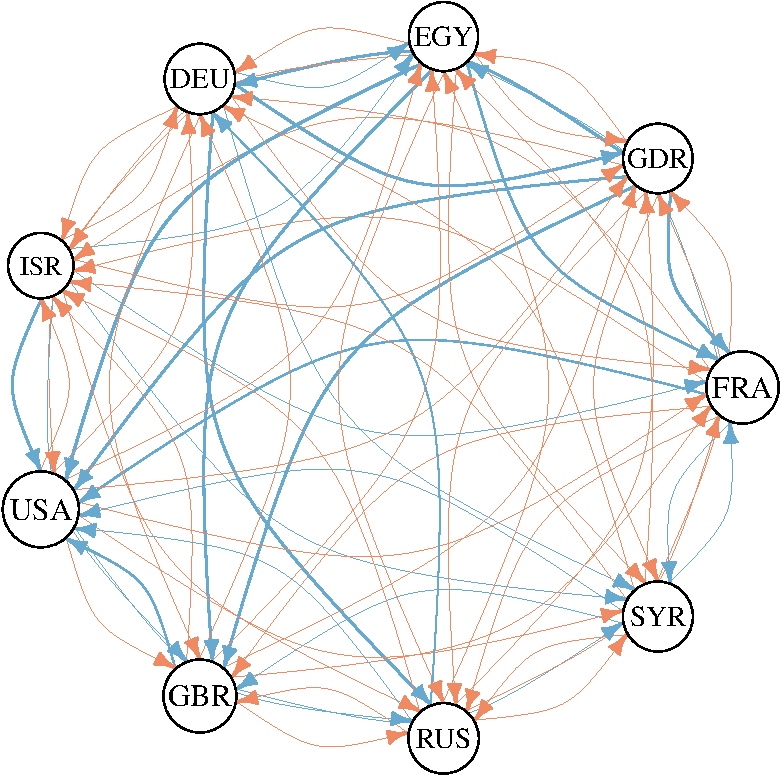
\includegraphics[width=.33\textwidth]{compNet_1972}
		\label{fig:comp72}} & 

	\subfloat[sub1][Compliance: 1992]{
		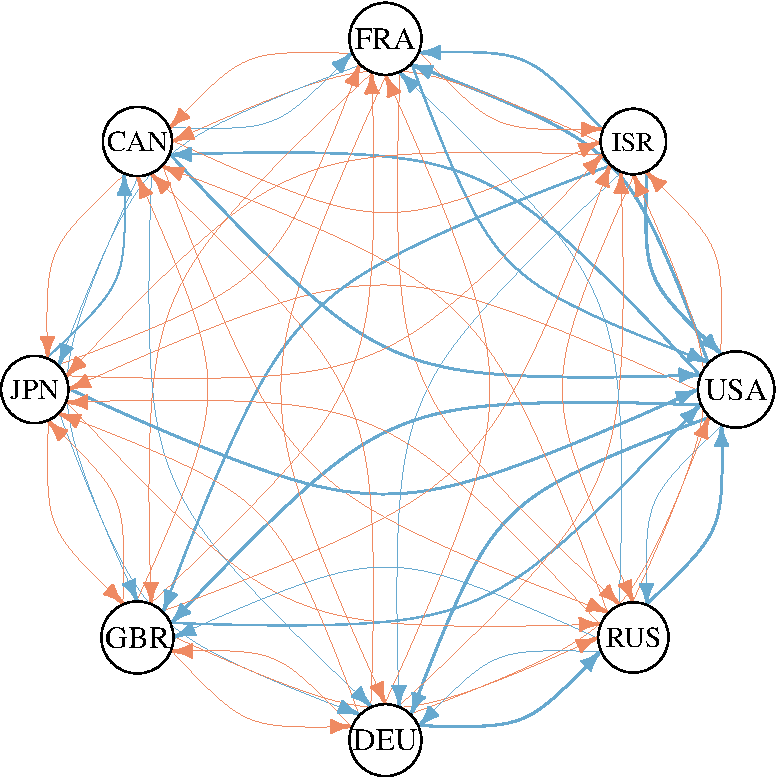
\includegraphics[width=.33\textwidth]{compNet_1992}
		\label{fig:comp92}} & 

	\subfloat[sub1][Compliance: 2012]{
		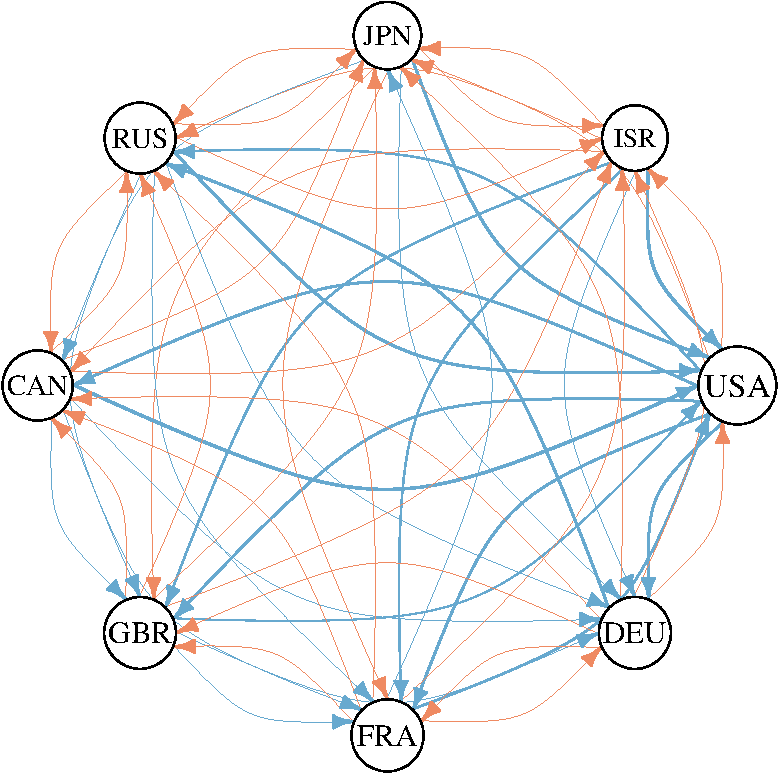
\includegraphics[width=.33\textwidth]{compNet_2012}
		\label{fig:comp02}}

	% \subfloat[sub1][Sanction: 1972]{
	% 	\includegraphics[width=.33\textwidth]{sancNet_1972}
	% 	\label{fig:sanc72}} & 

	% \subfloat[sub1][Sanction: 1992]{
	% 	\includegraphics[width=.33\textwidth]{sancNet_1992}
	% 	\label{fig:sanc92}} & 

	% \subfloat[sub1][Sanction: 2012]{
	% 	\includegraphics[width=.33\textwidth]{sancNet_2012}
	% 	\label{fig:sanc02}}

	\end{tabular}
	\label{fig:recipNet}
\end{figure}
\FloatBarrier

We extend this intuition to our second key measure, \textit{sanction reciprocity}. Following the same idea as compliance reciprocity, this is a measure of how often a target state has received sanctions from the senders of any given sanction case -- relative to all other sanction interactions of states. The intuition behind this measure is to capture the concept of creating expectations of resolve: states who have been sanctioned multiple times by a sender state are likely to build up a willingness of resistance and not cooperation.  This suggests that states receiving sanctions from those with whom they have been sanctioned before are likely to more slowly comply to those states. 

The basic insight is that states whom continually respond to sanctions by sending sanctions of their own are signaling more conflictual rather than cooperative behavior over time. This endogenously formed strategic environment is a dominating factor for the initiation of sanction compliance. Thus, in a world of changing information and strategic incentives, a country will not continue to repetitively comply to a partner state simply out of perceived strategic ties. Countries require continuous signals to build trust and cooperation over time and to maintain a shared understanding of strategic importance to one another. For this reason, we argue that reciprocity is an essential component endogenous to the strategic environment whereby an increase in reciprocity results in an increase in the likelihood of sanction compliance. 
